% Chapter 6
\section*{Preface}
In this chapter, performance of AIBs using various kinds of 2D and 3D materials as cathodes were explored. Graphitic carbon nitride (g-\ce{C3N4}), molybdenum trioxide (\ce{MoO3}) and electrospun tin oxide \ce{SnO2} fibers were tested as cathodes and their results have been reported. Prussian blue, which is a three-dimensional (3D) metal-organic framework (MOF), was also investigated as a cathode material. The most successful cathodes have been reported previously in Chapter 4 and 5. The other cathodes with their preliminary electrochemical tests have been summarised in this chapter. \footnote{All the materials used in this chapter, except \ce{MoO3}, are a part of collaborative work. the  materials were obtained from different sources to observe their performance as cathodes in non-aqueous AIBs.} 
\pagebreak
\chapter{Aluminium batteries using various 2D and 3D materials as cathodes} 
\label{chap6} 
Recent development in the field of two-dimensional (2D) materials has shown a lot of potential in the world of energy storage. Materials like graphene and its analogues, such as transition metal dichalcogenides, oxides, etc. have remarkable electrochemical properties. They can be used in most of the energy storage devices such as batteries, supercapacitors, redox flow batteries, photovoltaics etc. In addition to their tunable chemical and physical properties, 2D materials possess different crystallographic structures and elemental compositions. For this reason, they find immense use as electrode materials in electrochemical energy storage devices\cite{wang_graphene_2009,bonaccorso_graphene_2015}. In a review article on flexible LIBs that use graphene, Zhou \textit{et al.} showed that graphene and other 2D nanomaterials have a larger theoretical gravimetric capacity than their bulk counterparts \cite{zhou_progress_2014}. \\

\begin{figure}[h!]
  \centering
  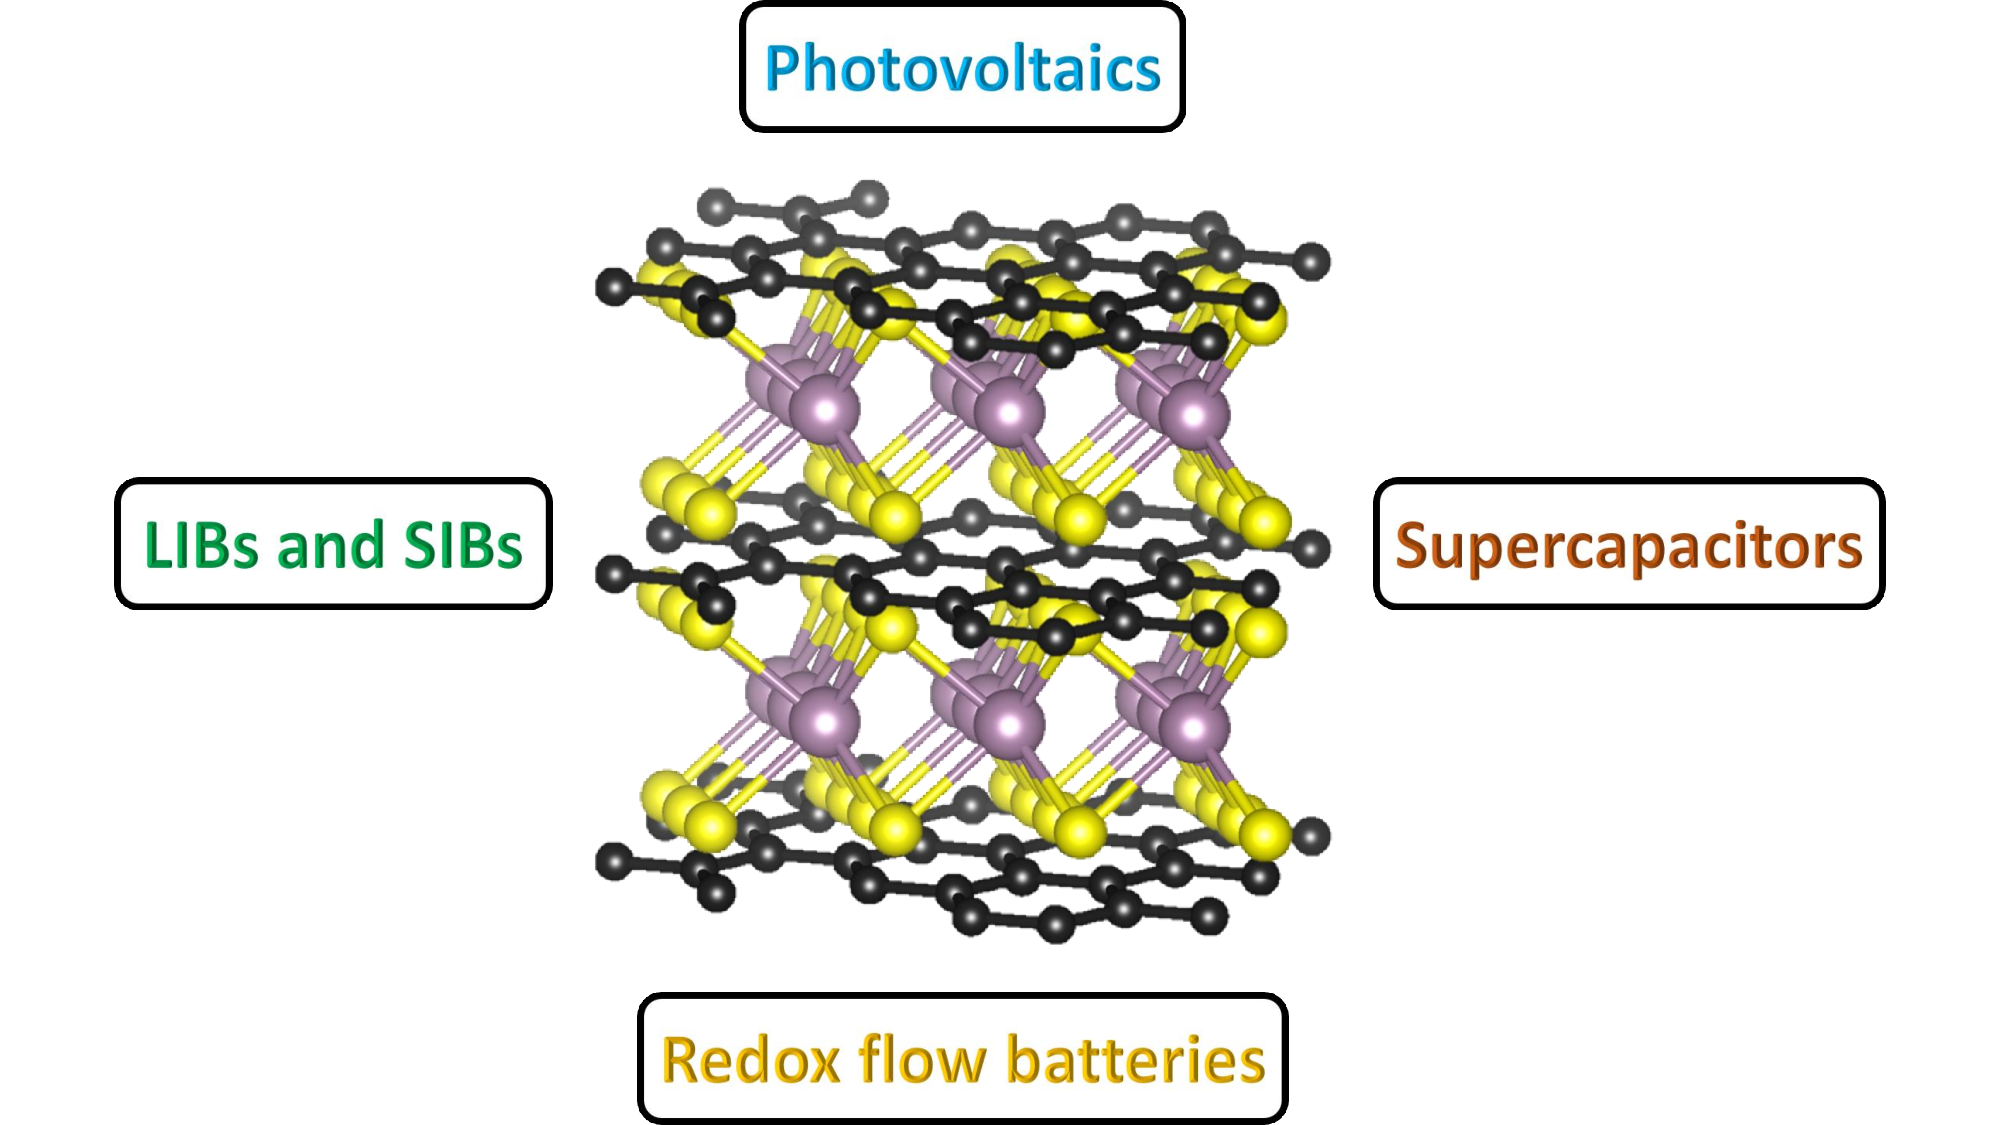
\includegraphics[width=\textwidth]{Figures/chap6fig/nanoTMDintro.pdf}
    \caption{An illustration of various applications of graphene and its analogues such as nanostructured molybdenum dichalcogenides.}
  \label{Figures/chap6fig:nanoTMDintro}
\end{figure}

\section{Tin oxide}

\subsection{Theory and background}
\begin{figure}[th!]
  \centering
  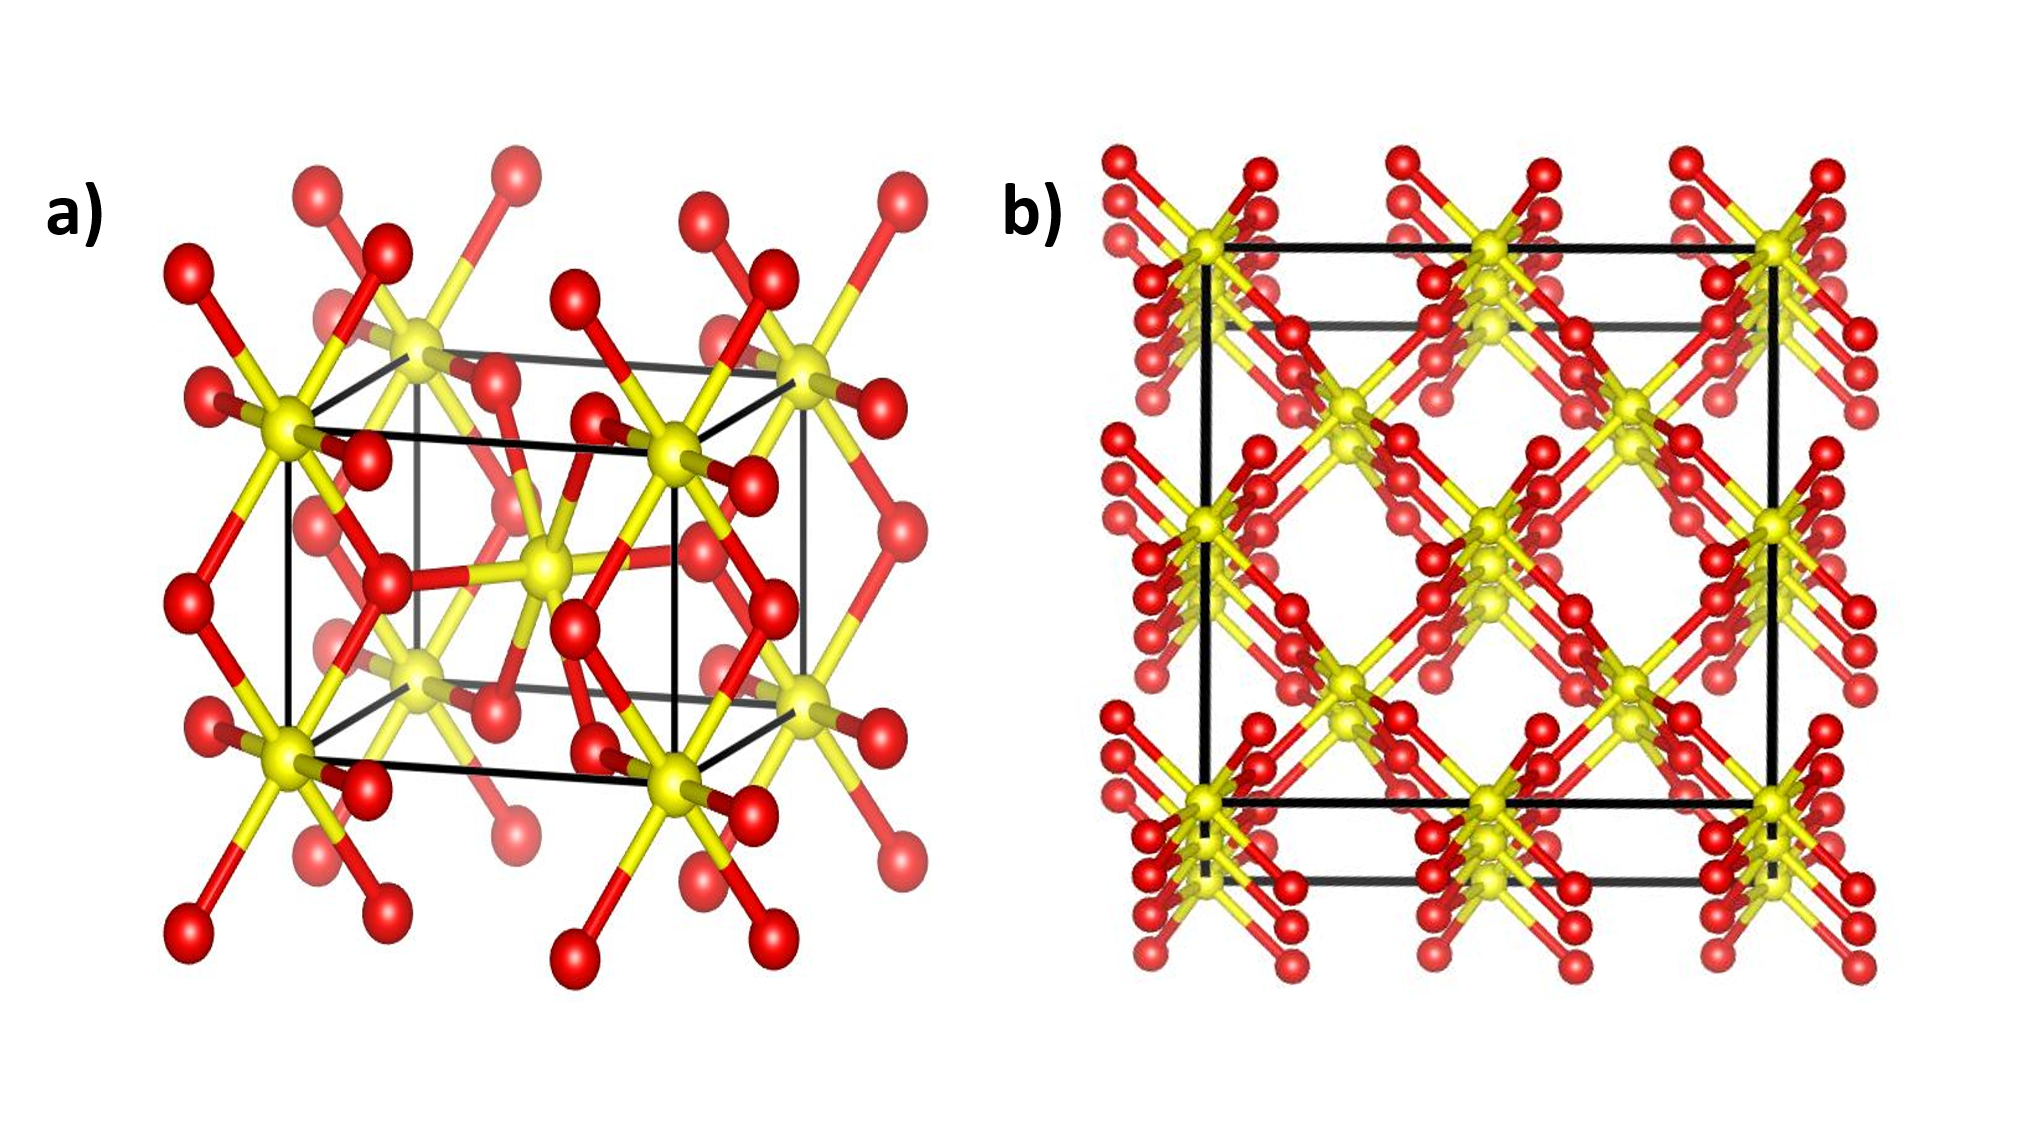
\includegraphics[width=0.75\textwidth]{Figures/chap6fig/SnO2crys}
    \caption{Crystal structure of \ce{SnO2}. Tetragonal unit cell with space group \textit{P4/nmm} and space group number 129.}
  \label{Figures/chap6fig:SnO2crys}
  \end{figure}
Due to its high theoretical capacity ($\approx$ 782mAh g$^{-1}$) and safe handling, \ce{SnO2} has been a popular choice as anodes in LIBs  \cite{idota_tin-based_1997}. Unfortunately, the major disadvantage of these materials is the large volume change during lithium insertion/extraction. Whittingham \textit{et al.} showed that pure tin foil (bulk) can be cycled at 600 mAh g$^{-1}$ for 10 to 15 cycles \cite{yang_anodes_2003}. However, the expansion and contraction of the anode during the cycles causes anode pulverisation and increases of the cell impedance (resistance). Consequently, due to the loss of electronic contact between the active material and the current collector, the capacity of the cells decreases after 15 cycles. Zhao \textit{et al.} reported the formation of \ce{Li2O} in addition to volume expansion when \ce{SnO2} was used as the anode, which further deteriorates the battery performance \cite{zhao_tin-based_2016}. Equation \ref{sn1} describes the formation of \ce{Li2O} and Equation \ref{sn2} describes the large volume variation that takes place due to formation of \ce{Li_{x}Sn} after Li atom reacts with Sn produced in the equations below.

\begin{equation}\label{sn1}
\ce{SnO2 + 4Li+ + 4e- -> 2Li2O + Sn} 
\end{equation}
\begin{equation}\label{sn2}
x\ce{Li + xe- + ySn -> Li_{x}Sn} 
\end{equation}

Since \ce{Li2O} is electrochemically inactive and non-conductive, it is also responsible for the large initial irreversible capacity. It has been reported that \ce{Li2O} can be decomposed via structural modifications of \ce{SnO2} on a nanoscale. Figure \ref{Figures/chap6fig:sno2pap} displays the performance of various kinds of \ce{SnO2} nanostructures (reported by Part \textit{et al.}) used in LIBs. The materials display a poor capacity retention even after 200 cycles.   

In their study on \enquote{Tin-based nanomaterials}, Zhao and her team assessed that adding carbonaceous materials to \ce{SnO2} increases its surface area, which makes more active sites available for lithiation \cite{navarrosuarez_2d_2018}. It also controls the volume expansion/shrinkage. Furthermore, it improves the conductivity of the material \cite{nowak_composites_2018}. Several nanostructured tin-based materials such as nanorods \cite{liu_direct_2009}, nanobelts \cite{duan_single_2005}, nanowires \cite{huang_situ_2010}, nanotubes \cite{wang_large-scale_2011} have been synthesised and tested as electrodes in energy storage devices which have shown improved performances from their bulk counterparts. 

\begin{figure}[th!]
\centering
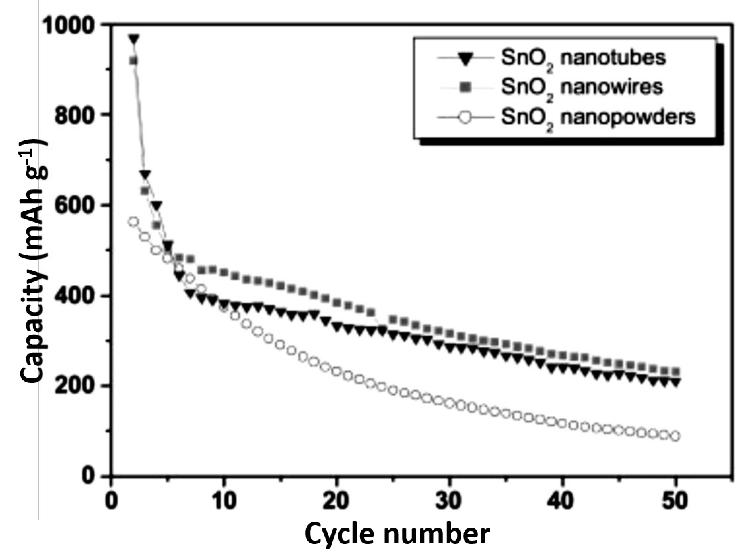
\includegraphics[width=0.75\textwidth]{Figures/chap6fig/sno2pap.pdf}
\caption{The cyclic performance of \ce{SnO2} nanomaterials in lithium-ion batteries up to the fiftieth cycle at a current density of 100 mA g$^{-1}$. Capacity of the materials decreases with every cycle due to expansion of \ce{SnO2}, which leads to cathode pulverisation and capacity fading \cite{park_effect_2008}.}
\label{Figures/chap6fig:sno2pap}
\end{figure}
\begin{figure}[th!]
\centering
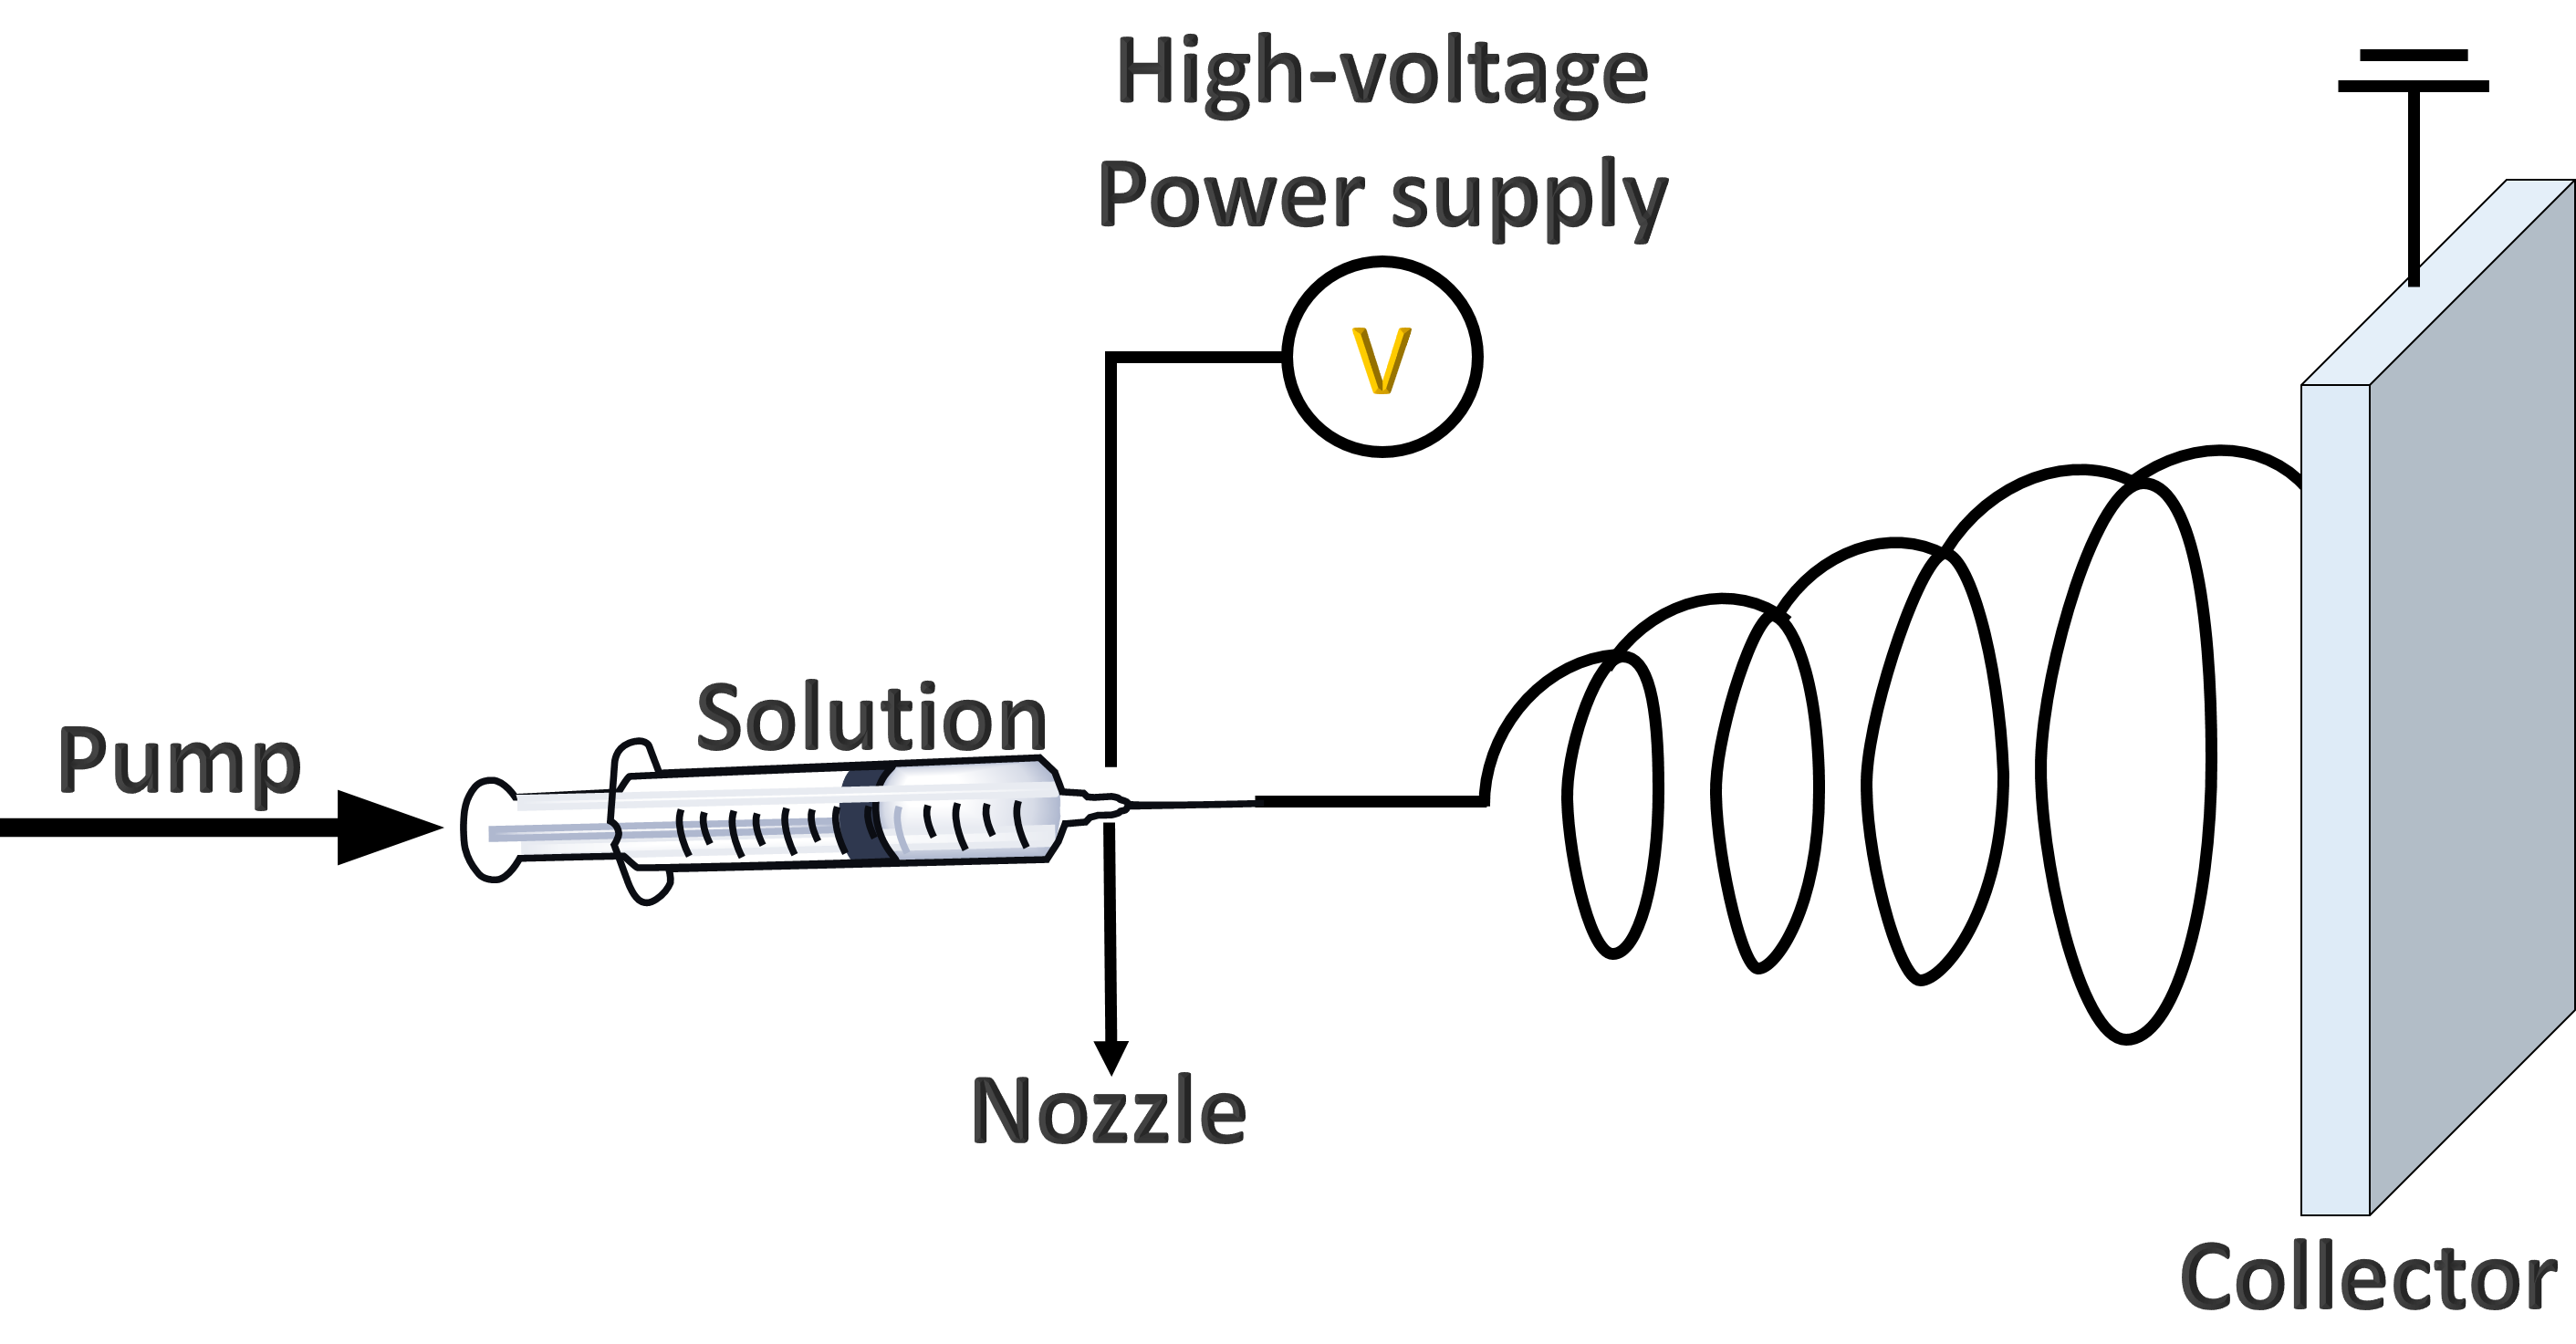
\includegraphics[width=\textwidth]{Figures/chap6fig/electrospinning}
\caption{A schematic illustration of an electrospinning setup.}
\label{Figures/chap6fig:electrospinning}
\end{figure}
\subsection{Experimental methods}
In this chapter, \ce{SnO2} fibers were obtained via  \enquote{electrospinning}. Dr. Sara Cavaliere, Lecturer at the University of Montpellier provided the electrospun \ce{SnO2} fibers, which were used as cathodes. Refer to Sections \ref{slurry}, \ref{catprep}, \ref{vac} and \ref{cellass} for cathode preparation and cell assembly methods. \\
\textbf{Electrospinning} is an electrostatic fiber fabrication technique. It uses an electrical force to produce polymer fibers with diameters ranging from 2 nm to a few $\mu$m. The techniques utilizes solution of both natural and synthetic polymers \cite{bhardwaj_electrospinning_2010}. The fibers obtained via electrospinning have smaller pores and a higher surface area than regular fibers produced by standard mechanical fiber-spinning technology \cite{huang_review_2003}. An electrospinning setup is illustrated in Figure \ref{Figures/chap6fig:electrospinning}. The topography and orientation of the fibers can be controlled by modifying parameters such as voltage, pump speed or nozzle thickness in the electrospinning setup.

\subsection{Results and discussion}
To evaluate the electrochemical properties, the Al/\ce{SnO2} cell was charged and discharged at constant current between 0.2-2.35 V at current rates ranging from 50-1500 mA g$^{-1}$. Figure \ref{Figures/chap6fig:SnO2newCDC} displays the voltage vs. specific capacity plot of the AIB. The curves demonstrated a well defined discharge plateau at $\sim$ 0.55 V. CE of the cell decreased with every cycle and reduced to <60\% after 500 cycles. The discharge capacity also decreased after every cycle and reached a value of $\sim$10 mAh g$^{-1}$ after 500 cycles. It might be possible that electrospun fibers suffered repeated expansion and contraction during the cycles and that might have caused cathode pulverisation. Although distinct voltage plateaus indicate reversible redox processes taking place during charge and discharge, \ce{SnO2} failed to deliver a stable performance. To confirm its redox activity, cyclic voltammetry was performed and the resultant scans are displayed in Figure \ref{Figures/chap6fig:Sno2CV}. The CV exhibits a reduction peak at 0.45 V and an oxidation peak at 0.55 V, which match perfectly with the discharging voltage plateau observed at 0.47 V and charging voltage plateau at 0.55 V respectively.    
\begin{figure}[th!]
  \centering
  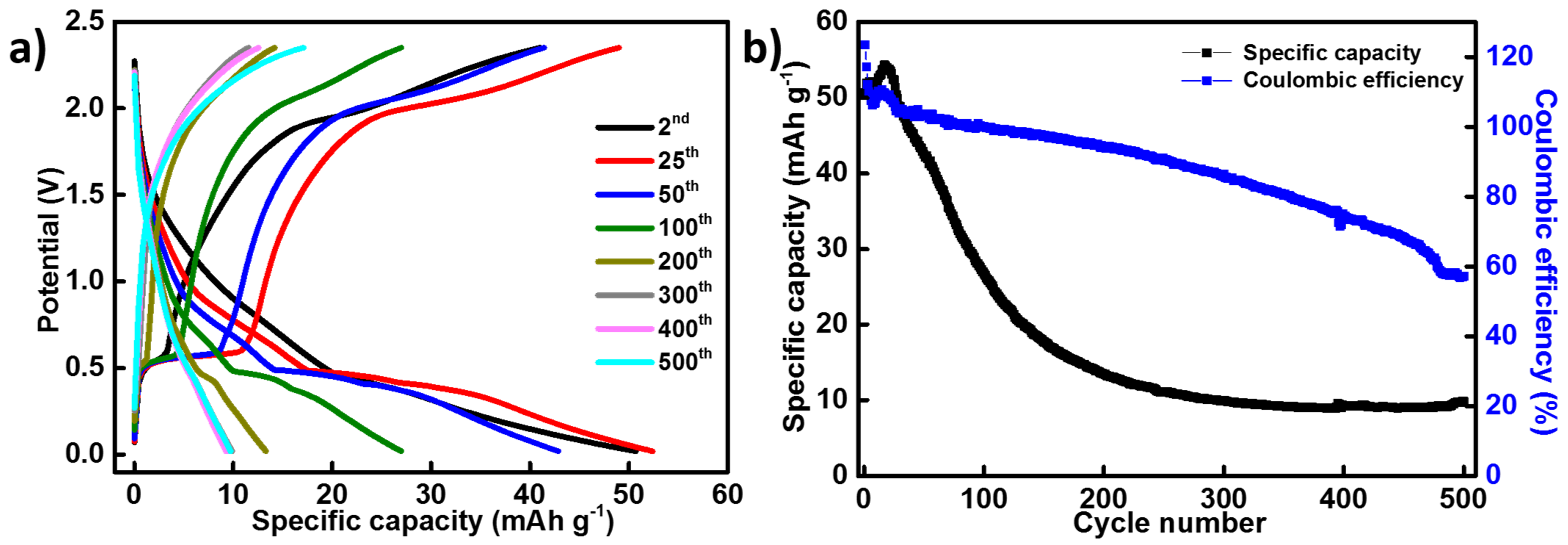
\includegraphics[width=\textwidth]{Figures/chap6fig/SnO2newCDC}
    \caption{a) Galvanostatic charge and discharge curve of an Al/\ce{SnO2} cell at the current rate of 40 mA g$^{-1}$. b) Long-term stability test of the cell.}
  \label{Figures/chap6fig:SnO2newCDC}
\end{figure}
However, the X-ray diffraction patterns in Figure \ref{Figures/chap6fig:SnO2XRD} look alike after charge and discharge. A shoulder develops in the charged and discharged cathodes at 2$\theta$ value of 22$^{\circ}$, which was absent in the pristine sample. Sharp Bragg peaks correspond to the crystalline phase and the broad bump under the peaks at 22$^{\circ}$ and  34$^{\circ}$ observed in the charged cathode corresponds to the amorphous state of the same material. Furthermore, the peak at 2$\theta$ value of 51$^{\circ}$ (\textit{211}) in the pristine sample, splits into two after charge. The peak splitting might suggest formation of another crystal structure or presence of secondary phase that was formed during charge. SEM images in Figure \ref{Figures/chap6fig:SnO2SEM} display the cathode morphology before and after cycles and a few fibers show signs of damage (Figure \ref{Figures/chap6fig:SnO2SEM} c) after charge/discharge. 

\begin{figure}[th!]
  \centering
  
\includegraphics[width=0.8\textwidth]{Figures/chap6fig/Sno2CV}
    \caption{Cyclic voltammogram of an Al/\ce{SnO2} cell with an oxidation peak observed at 0.6 V and reduction peak at 0.5 V against Al/\ce{Al^3+} within the voltage window of 0.2-2.35 V.}
  \label{Figures/chap6fig:Sno2CV}
\end{figure}
\begin{figure}[th!]
  \centering
  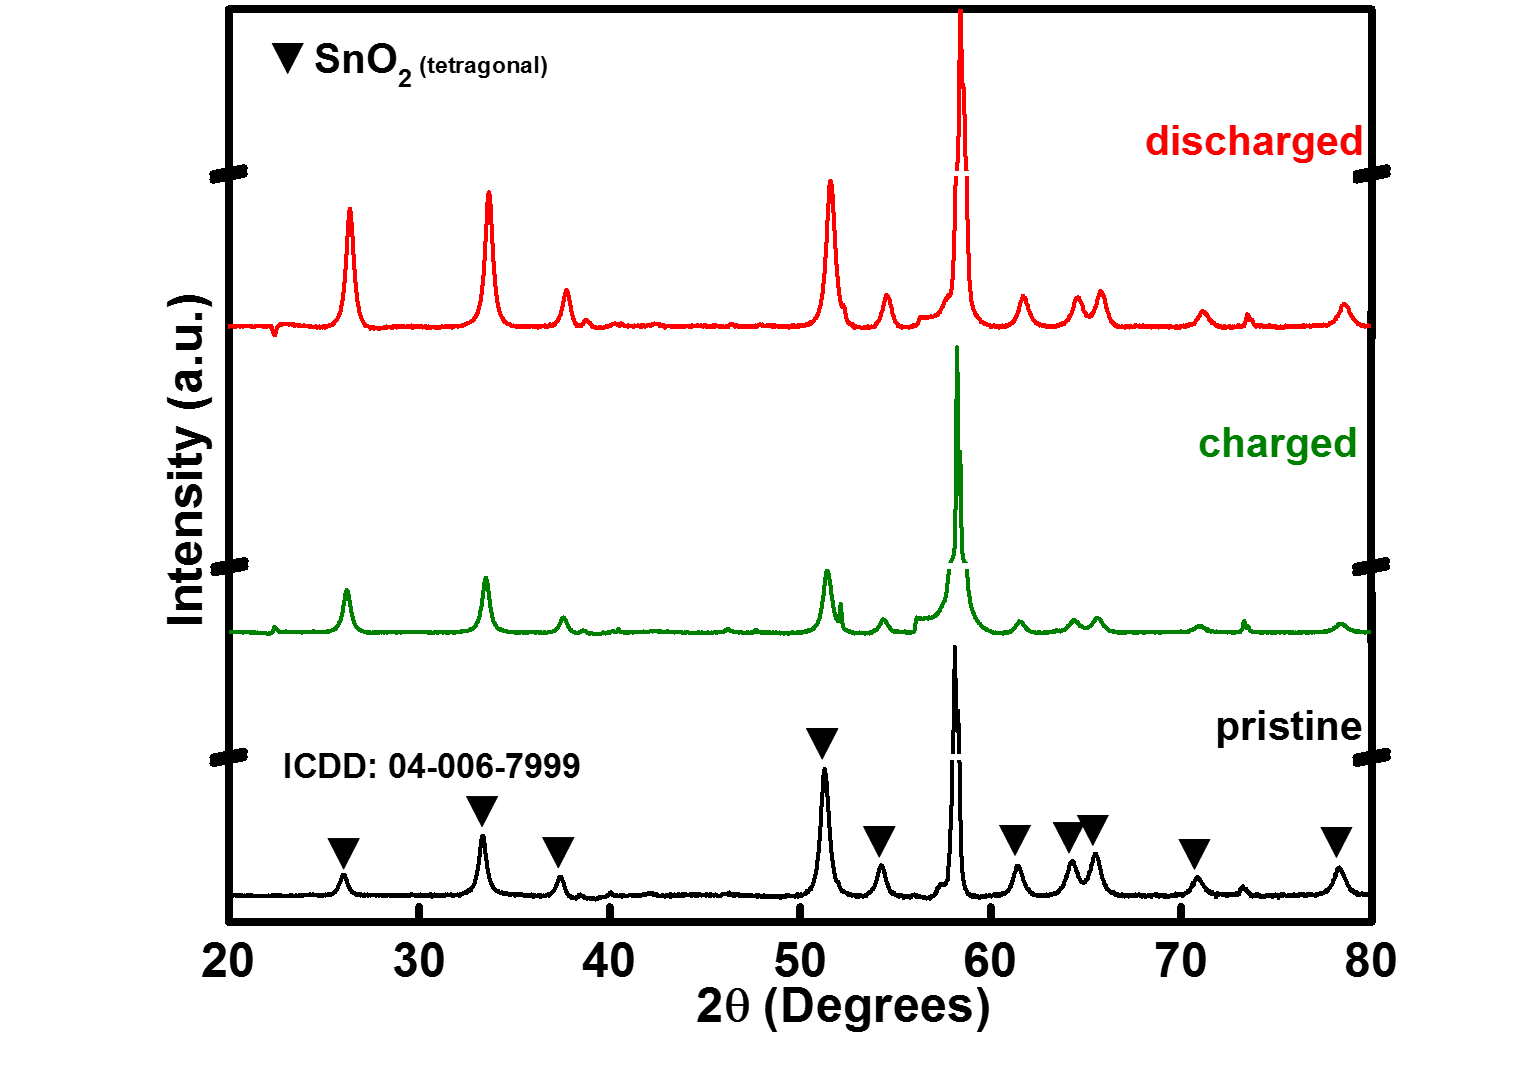
\includegraphics[width=0.8\textwidth]{Figures/chap6fig/SnO2XRD}
    \caption{\textit{Ex-situ} X-ray diffraction patterns of \ce{SnO2} cathode in a pristine (black), charged (green) and discharged (red) state.}
  \label{Figures/chap6fig:SnO2XRD}
\end{figure}
\begin{figure}[th!]
\centering
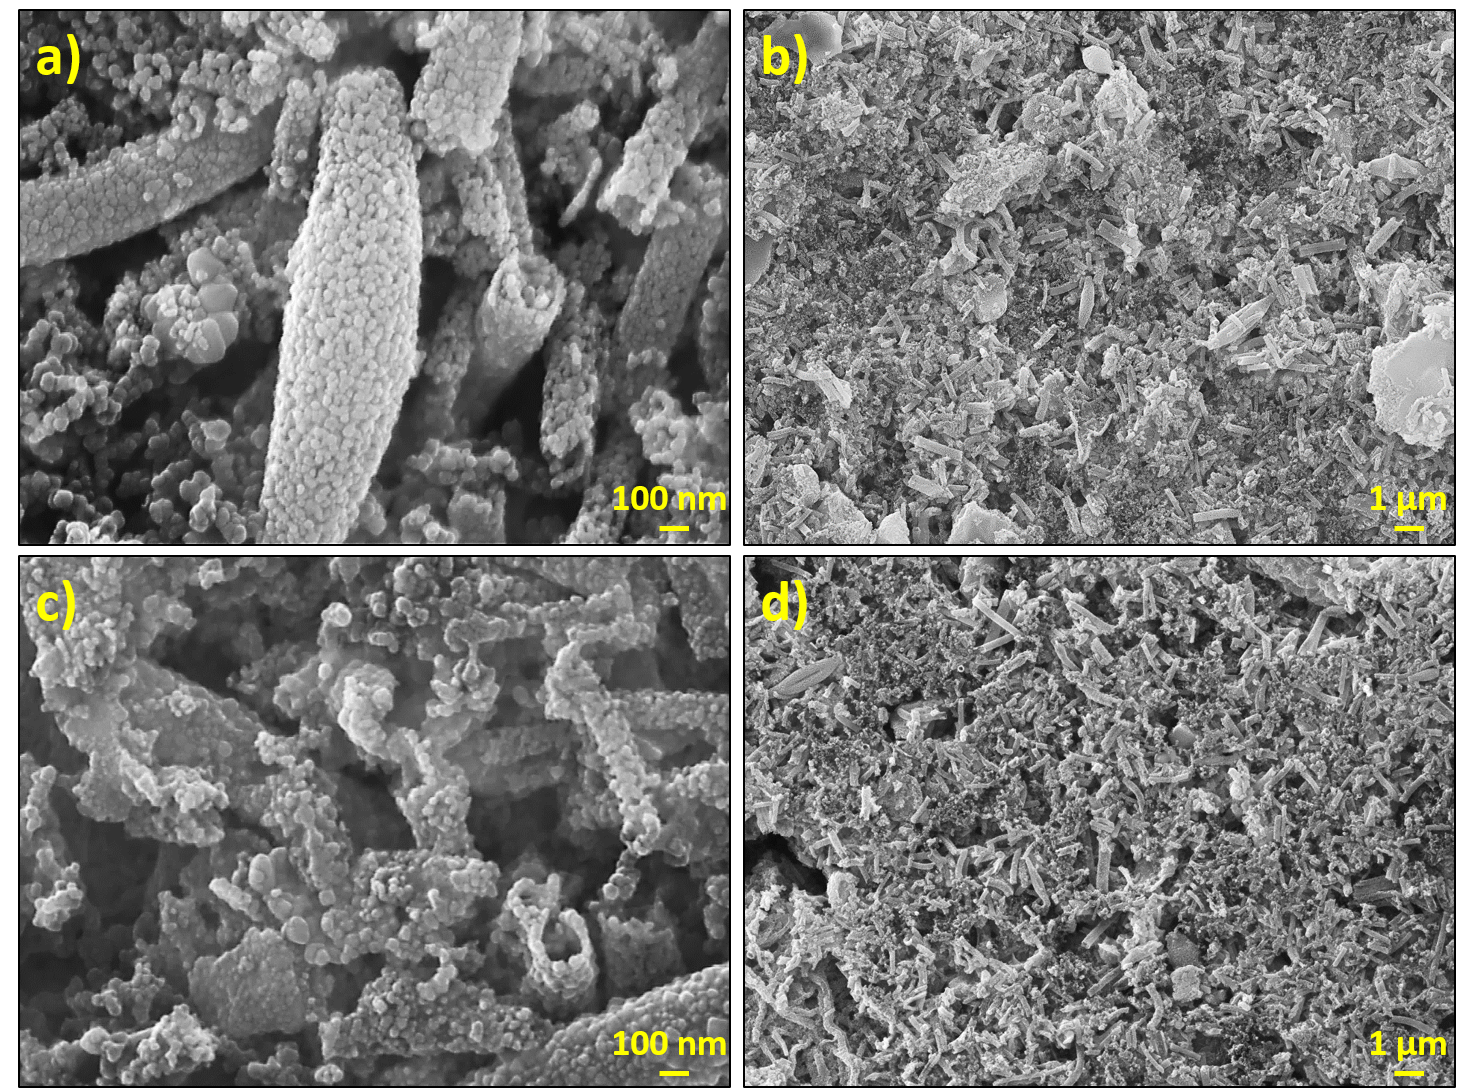
\includegraphics[width=\textwidth]{Figures/chap6fig/SnO2SEM}
\caption{SEM images of a,c)pristine and b,d) cycled \ce{SnO2} cathode.}
\label{Figures/chap6fig:SnO2SEM}
\end{figure}
\subsection{Summary}
Further analysis such as \textit{in-situ} XRD or an \textit{ex-situ} XPS analysis of the charged and discharged cathodes is needed to investigate whether \ce{SnO2} follows a similar type of charge storage in AIBs as it does in LIBs. It would be interesting to find out whether new complexes are being formed after \ce{AlCl4-} anions interact with \ce{SnO2} during charge/discharge cycles and the material follows a conversion-type reaction mechanism instead of ion-intercalation or both. Redesigning \ce{SnO2} fibers using materials that might make it more robust and eventually solve its problem of poor capacity retention. It is suggested that mixing the active material with carbon-based materials or making \ce{SnO2} hybrids (as suggested above for other battery systems) might improve the battery voltage. 


\section{Molybdenum trioxide}
\subsection{Theory and background}

 \begin{figure}[th!]
  \centering
  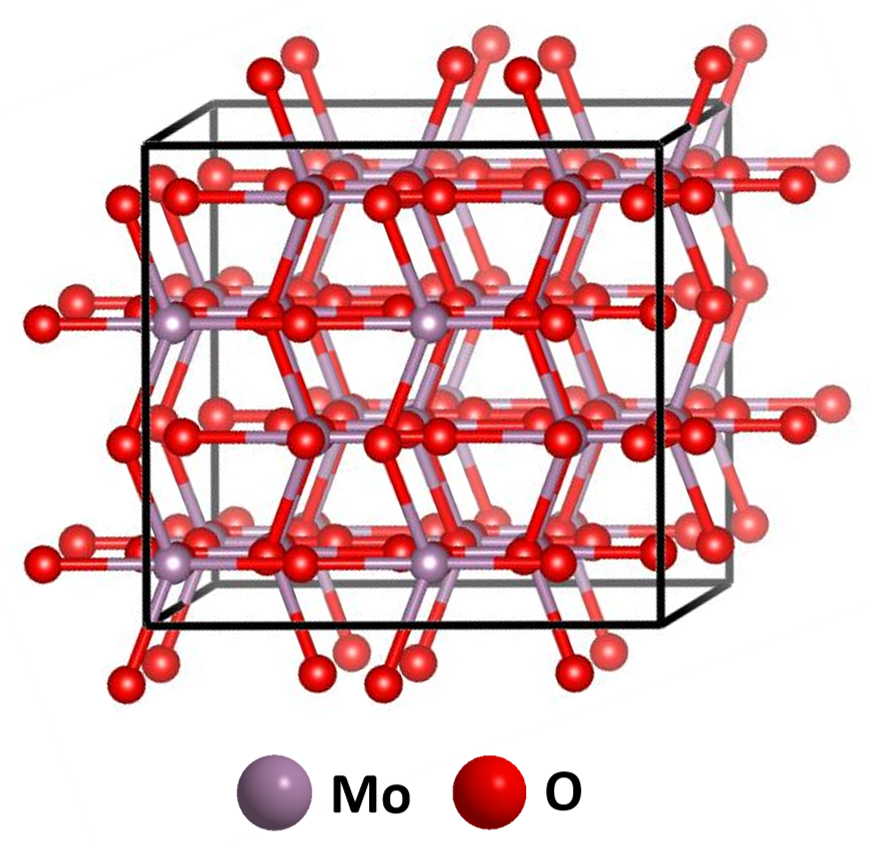
\includegraphics[width=\textwidth]{Figures/chap6fig/MoO3crys}
    \caption{Crystal structure of \ce{MoO3}.}
  \label{Figures/chap6fig:MoO3crys}
\end{figure}

Molybdenum trioxide (\ce{MoO3}) is an intermediate formed during production of molybdenum metal. It has a layered orthorhombic arrangement and contains four formula units of \ce{MoO3} per unit cell. The single sheet adopts a bi-layer structure with both sides of the surface terminated with oxygen atoms. The crystal structure of \ce{MoO3} is illustrated in Figure \ref{Figures/chap6fig:MoO3crys}. Due to its layered structure, \ce{MoO3} has been popularly used as an electrode material in LIBs \cite{wu_mixed_2017,li_vapor-transportation_2006,tsumura_lithium_1997}. Tsumura and Chen \textit{et al.} showed that the intercalation of \ce{Li+} ions and the resulting redox reactions resulted in capacities ranging from 200-400 mAh g$^{-1}$ \cite{tsumura_lithium_1997,chen_fast_2010,zhou_-moo3_2010}. As one of the earliest studied host materials for \ce{Li+} insertion, $\alpha$-\ce{MoO3} can accommodate $\sim$ 1.5 lithium per Mo atom. Lithiated \ce{MoO3} (\ce{LixMoO3}) displayed good electronic conductivity and high \ce{Li+} mobility. In 2006, Li and his team reported that the \ce{Li+} ions insert not only into the interlayer spacing between the \ce{MoO6} octahedron layers but also into the \ce{MoO6} intralayers \cite{li_vapor-transportation_2006,chen_fast_2010}. However, in 2011, Tao \textit{et al.} revealed that high concentrations of unsolvated \ce{Li+} in the host lattice sometimes causes irreversible structural changes resulting in poor cell performance \cite{tao_moo3_2011,li_theoretical_2014}. The reaction that takes place inside a LIB during discharge is given below in Equation \ref{moeq} \cite{li_vapor-transportation_2006}. 

\begin{equation} \label{moeq}
    \ce{xLi+ + MoO3 + xe- -> Li_{x}MoO3} 
\end{equation}
The above reaction is reversed during charge. \ce{MoO3} has also been used as a cathode material in aqueous AIBs as well \cite{joseph_hexagonal_2019, shakir_structural_2010, lahan_al3+_2019, lahan_active_2018}. Lahan and Das \textit{et al.} reported that the intercalation of \ce{Al^{3+}} cations was possible in orthorhombic \ce{MoO3}. However the performance was dependent on the electrolyte composition. They demonstrated that \ce{MoO3} stored more \ce{Al^3+} ions when \ce{AlCl3} was used instead of \ce{Al2(SO4)_3} and Al\ce{(NO3)_3} as the source of aluminium. It also minimized the cell polarization and improved the long-term stability of the cell. \ce{MoO3} cell achieved a specific capacity of 680 mAh g$^{-1}$ (highest reported value for any aqueous AIB) after its first discharge cycle. \\ 
Since \ce{MoO3} had never been tested as a cathode before in non-aqueous AIBs, it was used as an active material for this project. However, in 2018 (after the preliminary tests for this PhD thesis were completed), Nacimiento \textit{et al.} used layered-type $\alpha$-\ce{MoO3} as a cathode in non-aqueous AIBs using \ce{AlCl3}:EMIC in the ratio of 1.1:1.0 (slightly acidic melt) as the electrolyte. The maximum capacity achieved by those cells were 100 mAh g$^{-1}$, which decreased to 85 mAh g$^{-1}$ after 7 cycles. In addition, a rapid capacity decay was observed. The results obtained from those cells are displayed in Figure \ref{Figures/chap6fig:moo3pap}. After 11 cycles, the capacity decreased to 40 mAh $^{-1}$ at a very low current rate of 3 mA g$^{-1}$. 

\begin{figure}[th!]
\centering
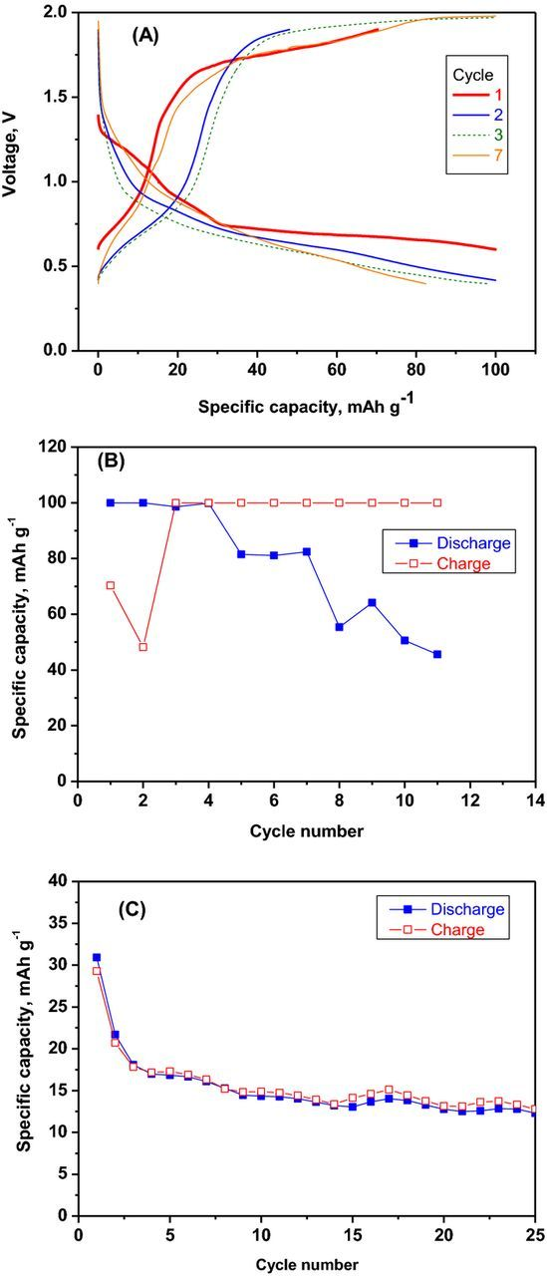
\includegraphics[width=0.5\textwidth]{Figures/chap6fig/moo3pap}
\caption{Galvanostatic experiments for \ce{MoO3} in an aluminum cell. A) Voltage-capacity curves and, B) corresponding capacity as a function of cycle number at current density 3 mA g$^{-1}$, and C) capacity as a function of cycle number at 10 mA g$^{-1}$ for 0.1-2.1 V of voltage limits \cite{nacimiento_exploring_2018}}
\label{Figures/chap6fig:moo3pap}
\end{figure}

\subsection{Experimental methods}
Molybdenum trioxide (ACS reagent, $\geq$99.5\%) was purchased from Sigma-Aldrich and used as received. Refer to Sections \ref{slurry}, \ref{catprep}, \ref{vac} and \ref{cellass} for cathode preparation and cell assembly methods. 

\subsection{Results and discussion}
At a high current rate of 1500 mA g$^{-1}$ (Figure \ref{Figures/chap6fig:MoO3cdcce} a), \ce{MoO3} achieved the highest capacity of $\sim$60 mAh g$^{-1}$ with CE>100\%. At various current densities and after 120 cycles, the cell managed to retain 75\% of its original capacity. Voltage bends were observed during charge at 2.0 and 1.7 V and a plateau was observed during discharge at 1.4 V. Discharge capacities at various current densities ranging from 50 mA g$^{-1}$ to 1500 mA g$^{-1}$ have been shown in Figure \ref{Figures/chap6fig:MoO3cdcce}. This cell performed better than Nacimiento's cell because it achieved higher capacities and displayed better capacity retention during discharge.  

\begin{figure}[th!]
\centering
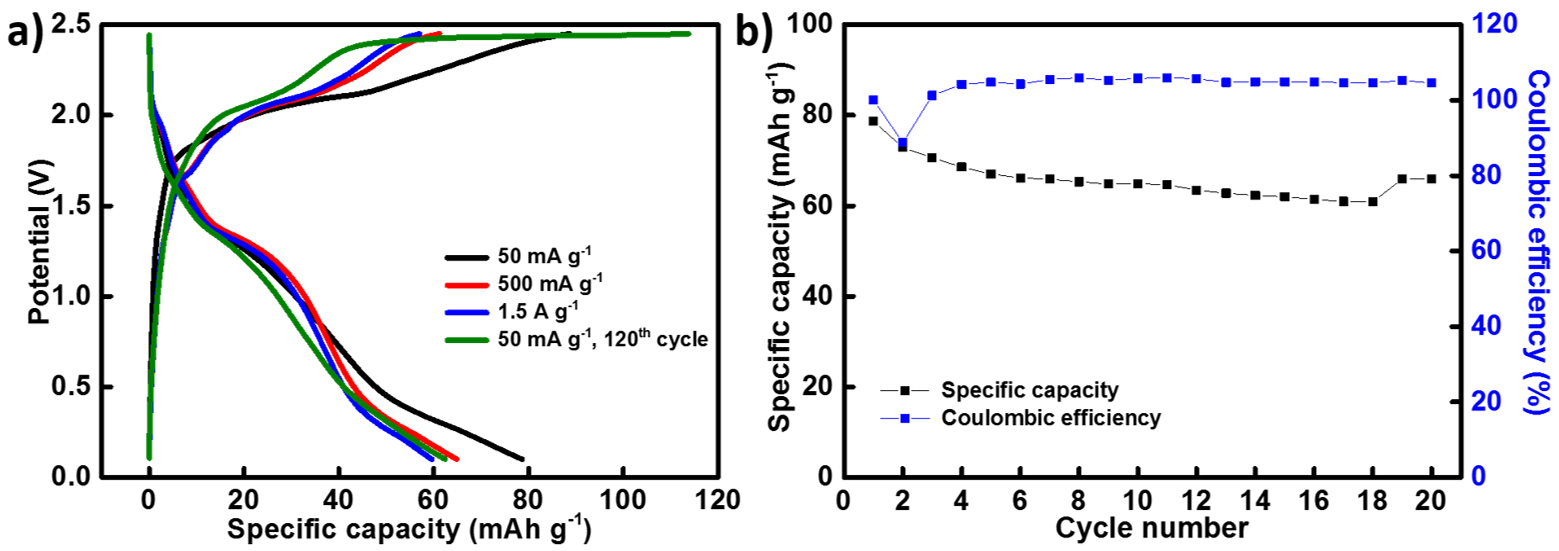
\includegraphics[width=\textwidth]{Figures/chap6fig/MoO3cdcce}
\caption{Charge/discharge cycles of an Al/\ce{MoO3} cell at various current rates.}
\label{Figures/chap6fig:MoO3cdcce}
\end{figure}

\subsection{Summary}
The electrochemical data suggests fast intercalation-based redox reactions similar to LIBs. With an energy density of $\sim$85 Wh kg$^{-1}$, this material shows a lot of potential for high-performing AIBs. 


\section{Graphitic carbon nitride}

\subsection{Theory and background}
Graphitic carbon nitride or g-\ce{C3N4} is a carbon-based material, which is highly stable under physiological conditions and displays semiconductive properties. The crystal structure can be regarded as N-substituted graphite framework consisting of $\pi$-conjugated graphitic planes formed via sp$^2$ hybridisation of C and N atoms. The inter-layer distance between the two stacks is 3.26\AA, and it is 2\% more densely packed than crystalline graphite \cite{zheng_graphitic_2012}. Due to N-atom substitution, the binding between two layers is strengthened, which decreases its inter-layer distance when compared to graphite (3.3 \AA). g-\ce{C3N4} is a low-cost metal free material with a high surface area \cite{zheng_graphitic_2012} and since the structure of g-\ce{C3N4} is analogous to graphite, it has been used for electrochemical energy storage applications. \\*
g-\ce{C3N4} has been used as a battery electrode material in LIBs, Li-\ce{O2}, Li-S, Zn-air, vanadium redox flow batteries and SIBs. Shah \textit{et al.} found that the presence of \enquote{pyridinic} N in g-\ce{C3N4} favors high \ce{Li+} intake and prohibits irreversible reactions. Therefore, nitrogen content and its type, highly influence the performance of g-\ce{C3N4} in LIBs \cite{shah_highly_2017}. \\*
Vanadium redox flow batteries on the other hand, have also used g-\ce{C3N4} as a catalyst. A typical vanadium redox flow battery consists of two electrolyte tanks with \ce{VO2+}/\ce{VO^{2+}} and \ce{V3+}/\ce{V2+} redox couples, two pumps and a battery cell. The electrochemical reactions take place at the electrode. For this reason, highly efficient catalysts are needed. Huang \textit{et al.} modified carbon felt (usually used as a catalyst in flow batteries) with g-\ce{C3N4} for catalyzing the redox reactions. This increased the energy efficiency (EE) of the cells to 87\%. In addition, Nafion membranes were replaced by g-\ce{C3N4} hybrids, such as sulfonated poly(ether ether ketone) SPEEK/g-\ce{C3N4} and oxidised g-\ce{C3N4} (OCN) ion membranes \cite{niu_novel_2017, wang_novel_2017}. An ion membrane separates the ion-pairs in the flow battery and accelerates the proton flow during charge/ discharge cycles. The g-\ce{C3N4} modified membranes not only improved the EE of the flow batteries but also increased its efficiency (CE: 97\% and EE: 83.6\%) when compared to Nafion (CE: 90\% and EE: 73.8\%). A good structural stability against strong oxidizing and acidic conditions was reported, which proved beneficial for these batteries. The acid-base pairs formed between -\ce{NH2} groups of g-\ce{C3N4} and sulfonic acid groups of SPEEK enhanced the vanadium ion permeability and its selectivity, and also improved the proton transport channel \cite{wang_novel_2017}. SPEEK/OCN membranes due to their high surface area and intrinsic stability of OCN contributed to decrease the vanadium ion permeability. The functional groups of OCN helped in improving the proton conductivity and improved the battery's performance. Due to all of the above-mentioned properties such as high surface area and structural stability that would prevent cathode pulverisation (as it was previously observed for other cathodes), g-\ce{C3N4} was tested as a cathode material for non-aqueous AIBs. It was speculated that the chloroaluminate ions would undergo a similar intercalation-type process that would be supported by the graphitic framework present in g-\ce{C3N4}.

\subsection{Experimental methods}
g-\ce{C3N4} that was synthesised using urea and was obtained from Associate Prof. Geoffrey Waterhouse from the University of Auckland. The material was used as received.  Kindly refer to Sections \ref{slurry}, \ref{catprep}, \ref{vac} and \ref{cellass} for cathode preparation and cell assembly methods. 

\subsection{Results and discussion}
Figures \ref{Figures/chap6fig:CNUcdccv} a and b show the charge/discharge curves and CV scan of g-\ce{C3N4} cell. The discharge capacity decreased from 160 mAh g$^{-1}$ to $\sim$100 mAh g$^{-1}$ after 120 cycles at the current rate of 50 mA g$^{-1}$. Figure \ref{Figures/chap6fig:CNUcdccv} a shows the discharge capacities at current densities ranging from 50 mA g$^{-1}$ to 1500 mA g$^{-1}$. The cell managed to achieve a capacity of 95 mAh g$^{-1}$ at 500 mA g$^{-1}$. A distinct charging plateau at 2.1 V and a slight bend during discharge at 0.6 V suggests the presence of reversible redox reactions. However, the capacity decreased to almost zero at 1500 mA g$^{-1}$, which implies that the current was too high and the cell was unable to complete the reactions necessary for charge storage. 

\begin{figure}[th!]
\centering
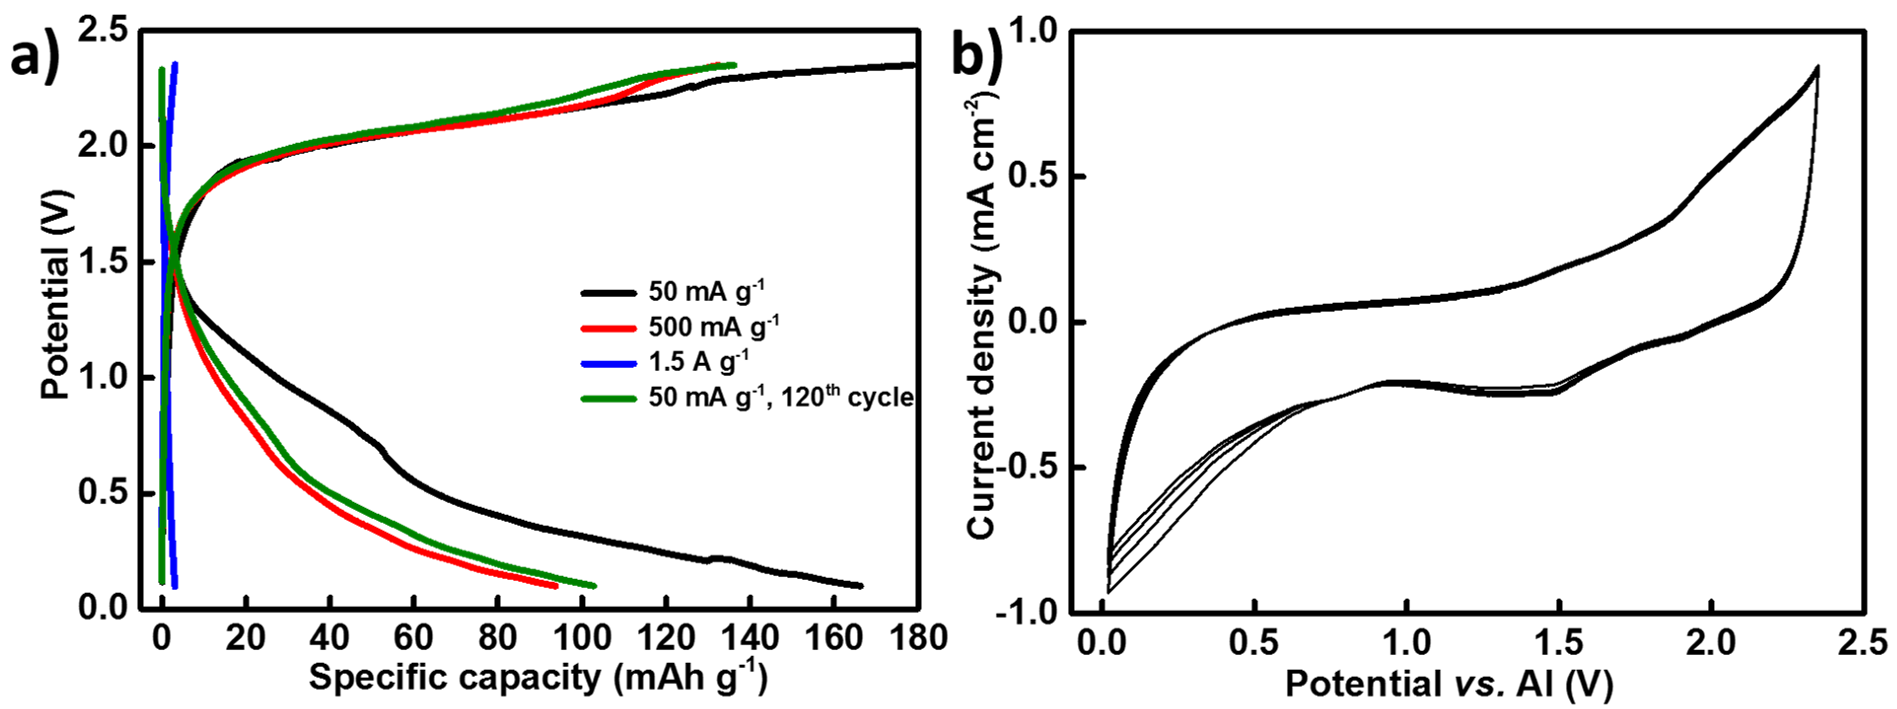
\includegraphics[width=\textwidth]{Figures/chap6fig/CNUcdccv}
\caption{a) Charge/discharge cycles of an Al/g-\ce{C3N4} cell at various current rates. The cell managed to retain 67\% of its original capacity after 120 cycles. b) Cyclic voltammogram of an Al/g-\ce{C3N4} cell; a reduction peak at 1.6 V was observed, which does not correspond to any of the voltage bends or plateaus observed in the charge/ discharge curves. }
\label{Figures/chap6fig:CNUcdccv}
\end{figure}

\subsection{Summary}
The storage performance of g-\ce{C3N4} in other battery systems was largely affected due to its large contact resistance and low band-gap \cite{shah_highly_2017}. Considerable efforts were made to improve its performance. Despite the fact that g-\ce{C3N4} has a more open structure than graphite, which should improve its \ce{Li+} intake and exchange capability, Luo \cite{luo_graphitic_2019} \textit{et al.} showed that the LIB using g-\ce{C3N4} anode displayed a capacity of 134.9 mAh g$^{-1}$ and an irreversible capacity loss of >98\% after 7 cycles. Veith and Hankel \textit{et al.} reported that reactions of lithium with g-\ce{C3N4} was responsible for the irreversible capacity loss \cite{veith_electrochemical_2013, hankel_lithium_2015}. Furthermore, they also reported that the replacement of C atoms with N atoms in the benzene ring was also proven to be responsible for its poor conductivity. These reasons might be valid for an AIB system as well since the material failed to retain its full capacity after 120 cycles. Nevertheless, there is still scope for improvement as new functional groups can be added to g-\ce{C3N4} that might improve its charge-storing capacity. The basic structural units used to build g-\ce{C3N4} are the triazine (\ce{C3N4}) and the tri-\textit{s}-triazine/ heptazine (\ce{C6N7}) ring shown in Figure \ref{Figures/chap6fig:c3n4}. The two structures possess different energetic stabilities because of the different electronic environments possessed by the N atoms and the size of the nitride pores. In 2016, Lin \textit{et al.} used density functional theory (DFT) calculations to demonstrate that the tri-\textit{s}-triazine based g-\ce{C3N4} was more stable and energetically favored. Hence, tri-\textit{s}-triazine is broadly recognized as the basic unit for the formation of the 2D sheets of g-\ce{C3N4}. Hence it is important to determine which one of the two rings formed the g-\ce{C3N4} structure. If it was triazine, modifications can be made so that tri-\textit{s}-triazine rings are formed that increase the charge-storing capacity of the cell. 

\begin{figure}[th!]
\centering
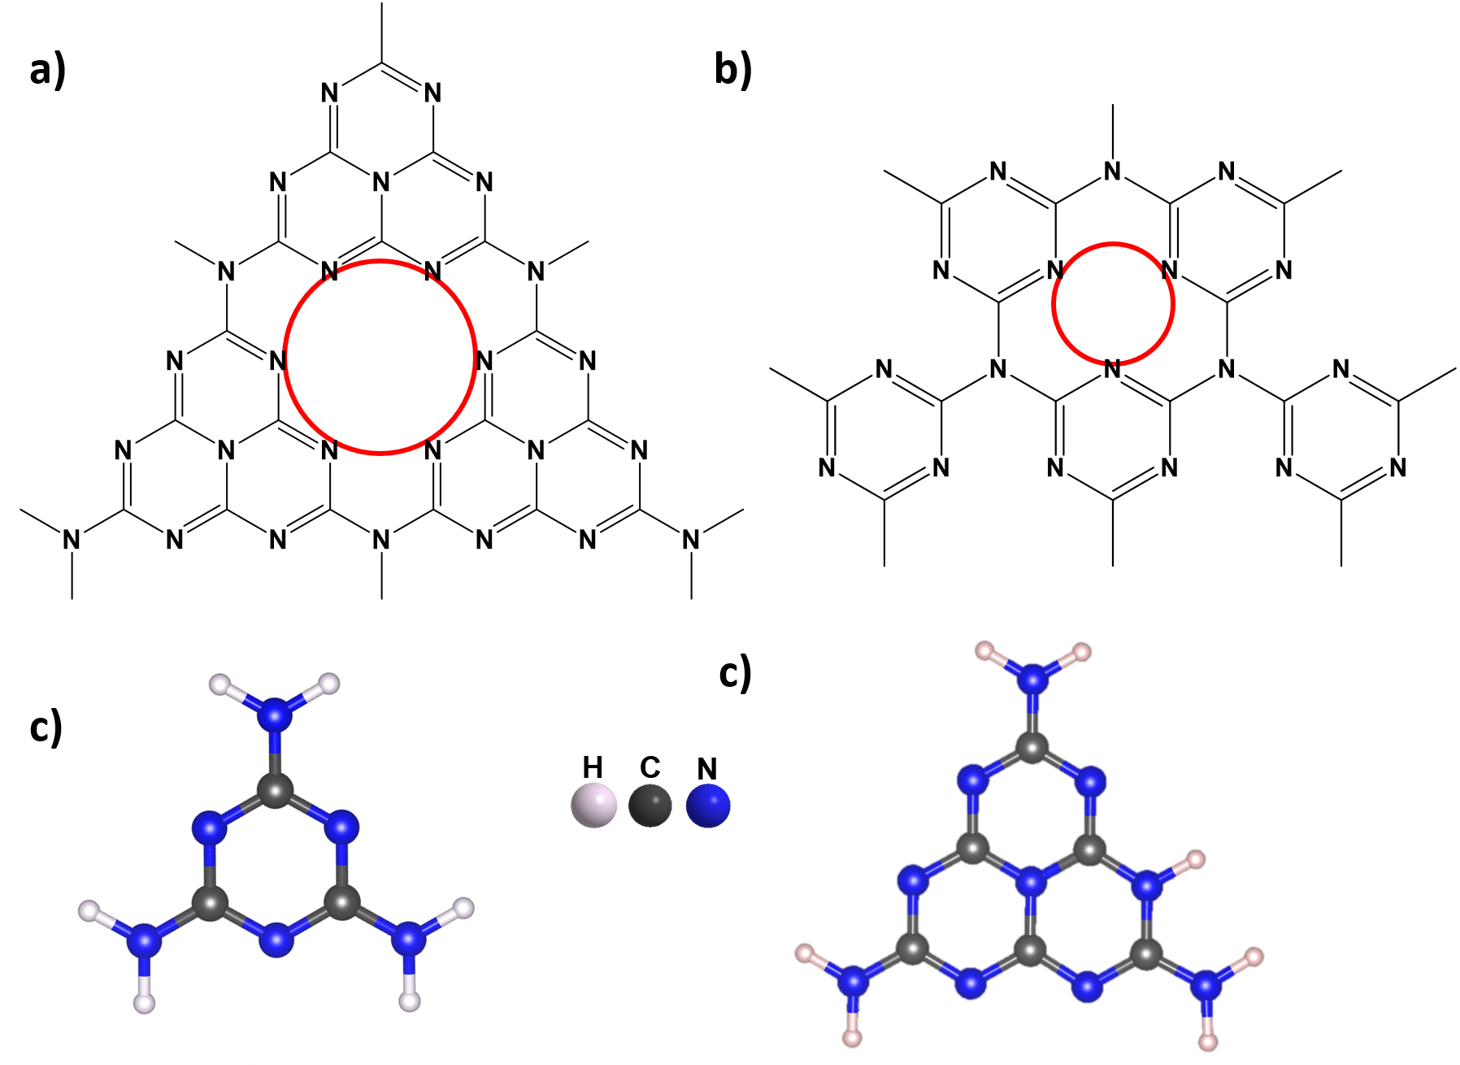
\includegraphics[width=\textwidth]{Figures/chap6fig/c3n4}
\caption{Structural motifs for graphitic-carbon nitride (g-\ce{C3N4}) molecules: a) fully condensed polyheptazine (tri-\textit{s}-triazine) \ce{C3N4} structure, and b) fully condensed triazine based \ce{C3N4} structure.}
\label{Figures/chap6fig:c3n4}
\end{figure}

\section{Prussian blue}

\subsection{Theory and background}

 \begin{figure}[th!]
  \centering
  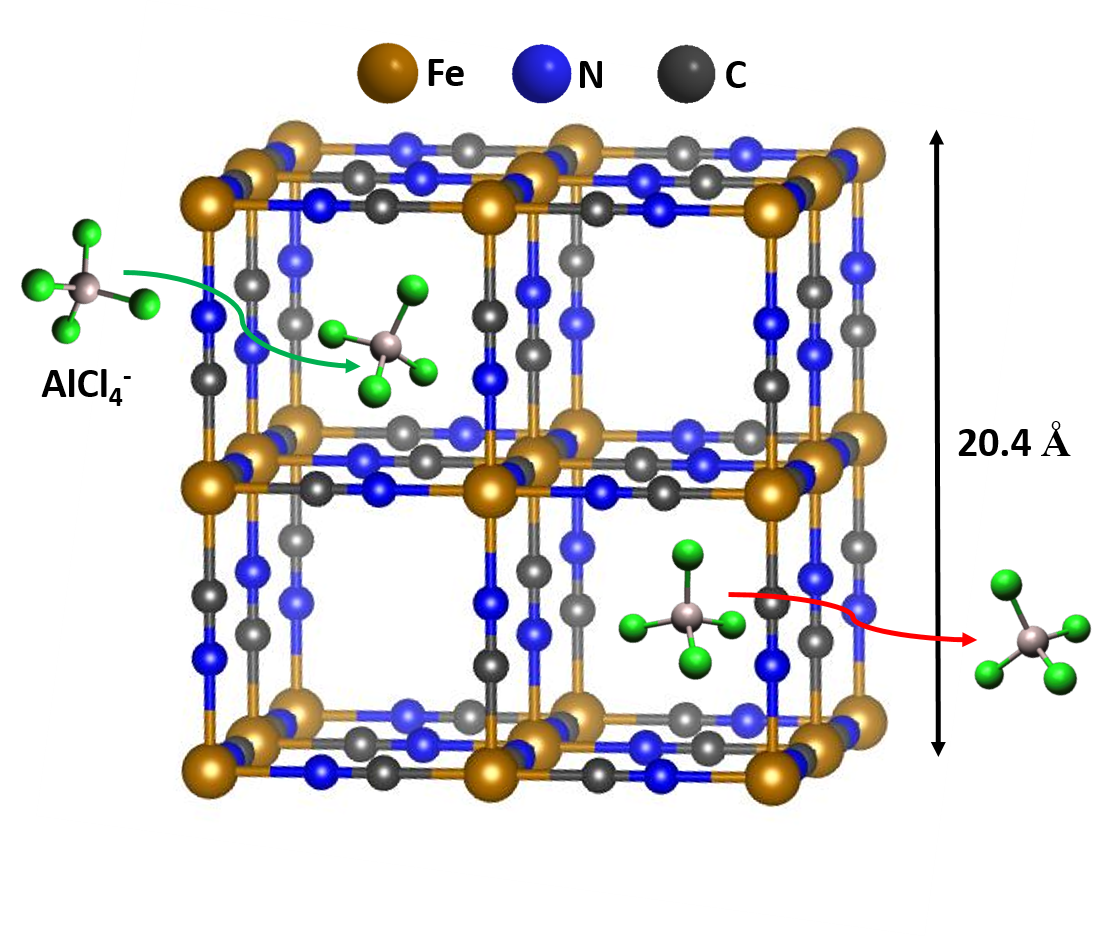
\includegraphics[width=\textwidth]{Figures/chap6fig/pbcrys}
    \caption{Crystal structure of Prussian blue. The voids present in the framework (20.4\AA) are spacious enough to allow the chloroaluminate ions (5.36\AA) to move in and out of it during charge and discharge. }
  \label{Figures/chap6fig:pbcrys}
\end{figure}

Prussian blue belongs to the family of metal-organic framework, also known as MOF. A MOF is a hybrid crystalline porous material. It consists of a regular arrangement of positively charged metal ions surrounded by organic molecules. A repeating cage-like structure is formed when metal cations form nodes that binds with an organic molecule's linker. MOFs have a large surface area (as high as 700 m$^{2}$ g$^{-1}$) due to their hollow structure. Figure \ref{Figures/chap6fig:pbcrys} displays the crystal structure of Prussian Blue, \ce{C18Fe7N18}. The structural uniformity and and the flexibility in their network topology, makes MOF an ideal battery material. Its open framework allow insertion of ions in the sub-cages. The structure has a number of redox sites present as each molecular formula contains two redox centres \ce{M^+2}/\ce{M^3+}, where M is any transition metal (Fe, Co, Ni, Mn, Cu, Zn). Presence of large lattice interstices and ionic channels renders a high specific capacity. The ability to tune MOFs along with its structural design, makes it different from the conventional porous materials. Due to their high surface area and and tailored pore-size, MOFs have been utilised as electrode materials in electric double layer capacitors or EDLCs, LIBs and SIBs. A Co-Zn MOF was designed by Diaz \textit{et al.} and it showed a typical EDLC behaviour in a non-aqueous electrolyte \cite{diaz_co8-mof-5_2012}. However, the specific capacitance for Co-Zn MOF was low. It was observed that cobalt-based MOF derived from Co\ce{(NO3)_2}, displayed pseudocapacitance behaviour suggesting presence of redox couples with an improved specific capacitance, instead of an EDLC behaviour. \\*
Recently, MOFs have been investigated as anode materials in LIBs \cite{li_shape-controlled_2006,han_synthesis_2012,zhao_metalorganic_2015}. To be used as anodes, the porous structure of MOFs allows reversible intercalation of \ce{Li+} ions during charge/discharge cycles. MOF-177 was the first MOF that was used as an anode material in LIBs \cite{li_shape-controlled_2006}. The material underwent a conversion-type reaction (metal ions present in the MOF get replaced by \ce{Li+} ions) inside the cell that destroyed its structure and consequently resulted in a poor cycling performance. Zhang \textit{et al.} investigated Prussian blue nanoparticles as anodes \cite{nie_prussian_2014}. The open-framework structure allowed rapid intercalation/ de-intercalation, where \ce{Li+} ions get stored in the MOF's cage-like structure and keep the structure intact. The cell achieved a reversible capacity of 300 mAh g$^{-1}$ and superior rate capability. Yagi and his group studied the lithiation mechanism in Prussian blue analogues (PBAs) \cite{yagi_eqcm_2014}. They reported that the redox reaction of PB might also proceed with the electrochemical adsorption/ desorption of \ce{PF6-} ions, which are the counter ions in the electrolyte. 
%A few other MOFs used in LIBs as anode materials have been listed in Table \ref{tableMOF}. 
PB has shown to have many applications in electrochemical energy storage. They can be used both in supercapacitors and in batteries. Based on the multiple valence of metal ions and open framework, novel electrode materials can be designed from MOFs and used in AIBs. For this reason, Prussian blue, a popular MOF, was tested as a cathode material in this project. 

%\vspace{0.5cm}
%\begin{table}
%\centering
%\caption{Summary of performances of MOFs used as anode and cathode materials in various energy storage devices.} \label{tableMOF}
%\begin{tabular}{ |p{1cm}|p{3.5cm}|p{2.2cm}|p{1.2cm}|p{1.5cm}|}
 %\hline 
%\textbf{Ref.} & \textbf{MOFs} & \textbf{Capacity (mAhg$^{-1}$)/ Capacitance (Fg$^{-1}$)} & %\textbf{Voltage (V)} & \textbf{Surface area (m$^{2}$g$^{-1}$)} \\ 
%\hline
%\cite{li_shape-controlled_2006} & {MOF 177} & 425 & 0.1-1.6 & -\\
%\cite{han_synthesis_2012} & Li/Ni-NTC & 1084 & 0.01-3 & -\\
%\cite{zhao_metalorganic_2015} & Asp-Cu nanofibers & 1255 & 0.01-3 & -\\
%\cite{wu_mof-templated_2013} & CuO & 1208 & 0.05-3 & -\\
%\cite{huang_metal-organic_2014} & \ce{Fe2O3}/\ce{NiCo2O4} & 1311 & 0.01-3 & -\\
%\cite{nagarathinam_redox-active_2012} & \ce{K2.5VO2}\ce{HPO4}\ce{C2O4} & 62 & 2.5-4.6 & -\\
%\cite{zhang_monitoring_2014} & Cu(2,7-AQDC) & 147 & 1.7-4 & -\\
%\cite{liu_metalorganic_2010} & NPC650 & 222 & - & 1521\\
%\cite{hu_porous_2010} & MC-A & 208 & - & 1674\\
%\cite{tang_thermal_2015} & NC/GC & 270 & - & 1276\\
%\cite{chen_high-performance_2013} & N-PC & 219 & - & 484\\
%\cite{banerjee_mof-derived_2014} & MOF-DC & 149 & - & 2714\\
%\hline
%\end{tabular}
%\end{table}
\subsection{Experimental methods}
Prussian blue was synthesised by another PhD student Fraser Hughson (part of Thomas Nann and Jim Johnston's group)  in Victoria University of Wellington. Refer to Sections \ref{slurry}, \ref{catprep}, \ref{vac} and \ref{cellass} for cathode preparation and cell assembly methods. 
\subsection{Results and discussion}
Figure \ref{Figures/chap6fig:pbcdccecv} displays the charge/ discharge curve exhibited distinct voltage bends and plateaus during discharge and charge at 1.8, 1.2 V and 0.6 V with a capacity reaching $\sim$140 mAh g$^{-1}$ after first 20 cycles. To investigate the rate capabilities of the battery, the cell was charged and discharged at various current densities ranging from 50-1500 mA g$^{-1}$. The specific capacities and CEs over 180 cycles at different current rates are shown in Figure \ref{Figures/chap6fig:pbcdccecv} b. At a high current density of 1500 mA g$^{-1}$, the capacity of the battery gradually decreased to 5 mAh g$^{-1}$. 

 \begin{figure}[tbh!]
  \centering
  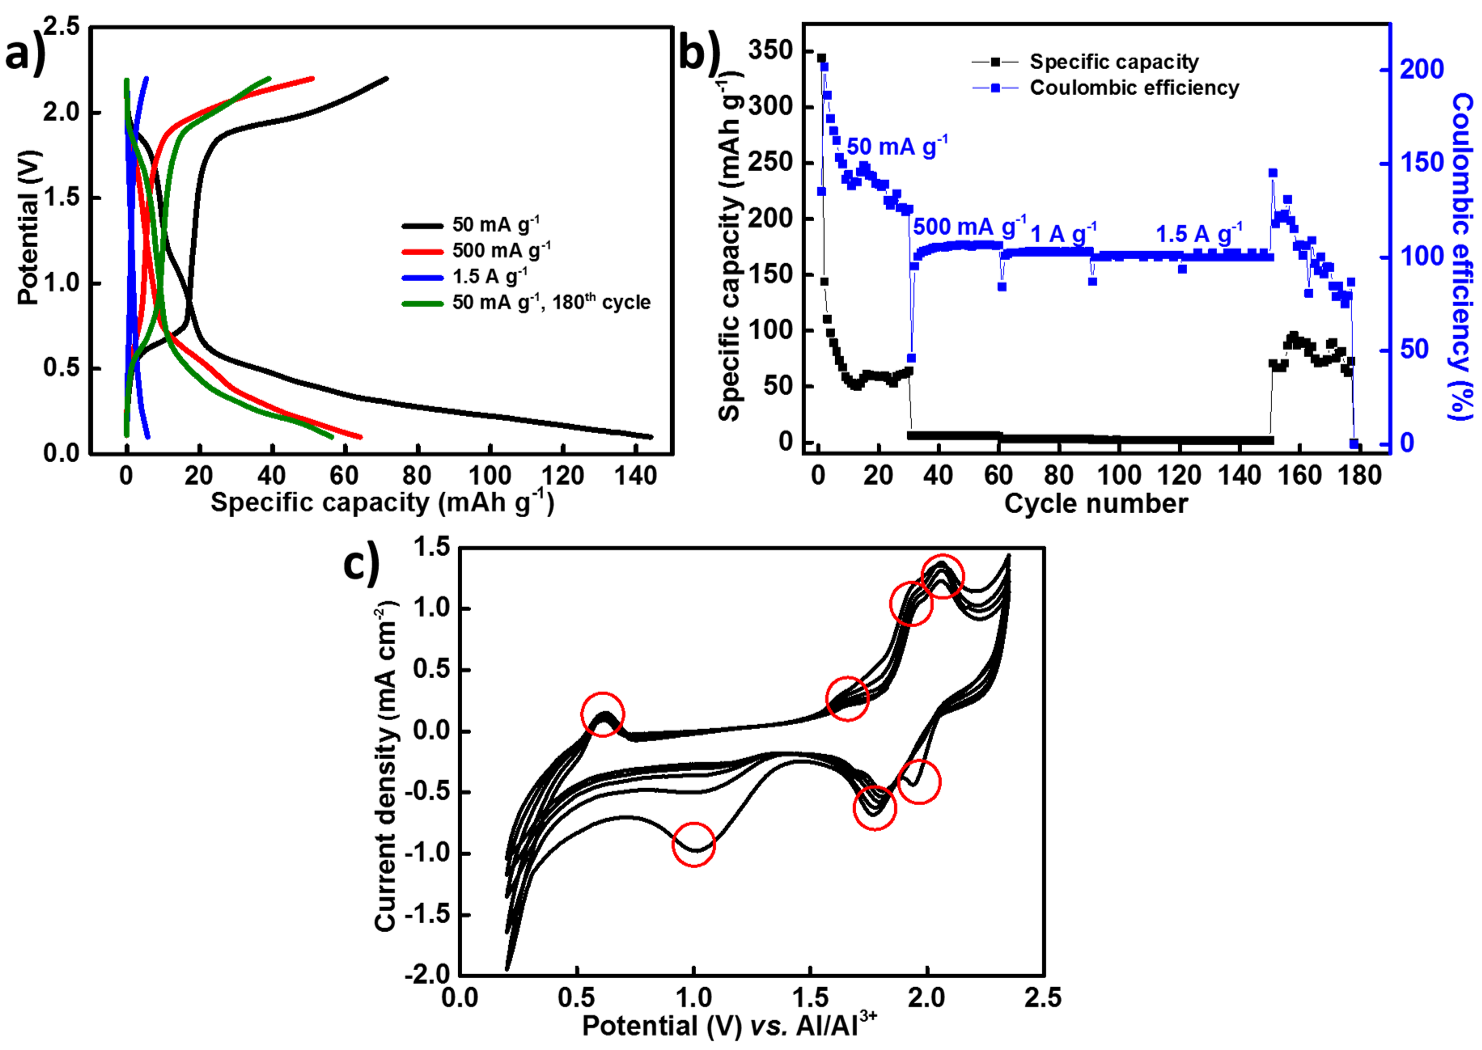
\includegraphics[width=\textwidth]{Figures/chap6fig/pbcdccecv}
    \caption{Galvanostatic cycle test of an Al/\ce{C19Fe7N18}, Prussian blue, cell in a two-electrode setup at various current rates. b) Long-term cell stability test at various current rates ranging from 50 to 1500 mA g$^{-1}$. c) CV curve of an Al/PB cell at a scan rate of 10 mV s$^{-1}$. The plateaus observed during charge at 0.6 and 1.8 V are almost identical to the oxidation peaks at 0.65 and 1.8 V. Voltage bend at 1.8 V during discharge corresponds to the sharp reduction peak at 1.8 V. Another oxidation peak at 2.15 V with a shoulder at 2.0 V }
  \label{Figures/chap6fig:pbcdccecv}
\end{figure}

\subsection{Summary}
In a review article by Lu Wang, it was reported that due to structural degradation, MOFs underwent large irreversible capacity losses and completed lesser number of cycles. This might be one of the reasons why the Al/MOF cell displayed a similar trend. However, they also proposed a number of possible solutions to improve the performance of MOFs as a battery material \cite{wang_metalorganic_2016}. Supposing that the cell undergoes conversion-type reaction, then the type of ligand in the MOF plays an important role because it determines if the MOF structure can be easily regenerated after every cycle. In case the cell undergoes an intercalation-type mechanism, MOF with a robust structure is highly desirable. Wang \textit{et al.} suggested that a metal ion with multiple valence states and low molecular weight ligands rich in functional groups promotes insertion of \ce{Li+} ions \cite{wang_metalorganic_2016}. Therefore, altering the current MOF i.e. \ce{C19Fe7N18} by using the above-mentioned techniques should certainly improve its performance in non-aqueous AIBs. 

\section{Conclusion}
In this chapter 2D cathode materials, owing to their special properties such as high surface area and ability to provide shorter ion diffusion path lengths, were tested as cathodes for non-aqueous AIBs.  
Supplemental research is required for an in-depth analysis of all the above-mentioned materials so that a comparative study can be made and a post-mortem analysis would also help in determining their mechanisms individually. The current chapter makes way for a number of future projects in the field of non-aqueous aluminium batteries, which will help in discovery of many more cathode materials for high-performing AIBs.  